\documentclass[a4paper,12pt,titlepage]{article}

\usepackage[german,ngerman]{babel}
\usepackage{fontspec}
\setmainfont{Calibri}
\usepackage{graphicx}
\usepackage{hyperref}
\usepackage{caption}

\begin{document}

\begin{titlepage}
    \centering
    \vspace*{2cm}
    {\LARGE\bfseries Automaten und formale Sprachen Blatt 5\par}
    \vspace{2cm}
    {\Large Jan Lucca Agricola (275867) \& Jakob Schulz (275258)\par}
    \vspace{2cm}
    {\large\today\par}
\end{titlepage}

\section{Aufgabe}
$L(G) = \{aba^n\, |\, n >= 0\}$\\
$L(G) = \{ab, aba, abaa, abaaa, abaaaa,...\}$
\section{Aufgabe}
$\Sigma = \{a,b\}\\
V = \{A,B, S\}\\
P = \{S \rightarrow Sa, S \rightarrow Ab, A \rightarrow Ba, B \rightarrow \epsilon\}$
\section{Aufgabe}
$L(G) = \{a^nb^m\, |\, n >= 0, m>= 1\}$\\
$L(G) = \{b, ab, aab, aabb, aabbb, aaab, aaabb, aaabbb, aaabbbb, aaaab,...\}$
\section{Aufgabe}
Die Grammatik G ist nicht vom Typ-3, weil sich beispielsweise ein Nichtterminal zu einem Terminal und zwei Nichtterminalen ableiten lässt $(S \rightarrow Sab)$\\
\\
\textbf{Äquivalente Typ-3-Grammatik:}\\
$G' = (\{S, A, B, C\}, \{a, b\}, P', S)\\
P' = \{S \rightarrow Ab, S \rightarrow Ba, A \rightarrow Sa, B \rightarrow Ca, C \rightarrow \epsilon\}
$
\section{Aufgabe}
$G = (\{S, A, B\}, \{a, b\}, P, S)\\
P = \{\\S \rightarrow Ab,\\ S \rightarrow Aa,\\ A \rightarrow Bb,\\ A \rightarrow Ba,\\ B \rightarrow Sb,\\ B \rightarrow Sa,\\ S \rightarrow \epsilon\\\}
$
\section{Aufgabe}
\subsection{Blatt 3 Aufgabe 2}
$G = (\{S, A, B, C, D\}, \{a, b\}, P, S)\\
P = \{\\
S \rightarrow Aa\\
A \rightarrow Ba,\\
A \rightarrow Bb,\\
B \rightarrow Ca,\\
B \rightarrow Da,\\
B \rightarrow Db,\\
D \rightarrow Aa,\\
D \rightarrow Ab,\\
C \rightarrow \epsilon\\
\}$
\subsection{Blatt 3 Aufgabe 3}
$G = (\{S, A, B, C\}, \{a, b\}, P, S)\\
P = \{\\
S \rightarrow Aa,\\
A \rightarrow Bb,\\
B \rightarrow Ca,\\ 
B \rightarrow Sa,\\
C \rightarrow \epsilon\\
\}$
\section{Aufgabe}
\subsection{Grammatik}
Grammatik $G = (\{S\}, \{(, )\}, P, S)\\
P = \{\\
S \rightarrow (S),\\
S \rightarrow SS,\\
S \rightarrow \epsilon\\
\}$
\subsection{Ableitungsbäume}
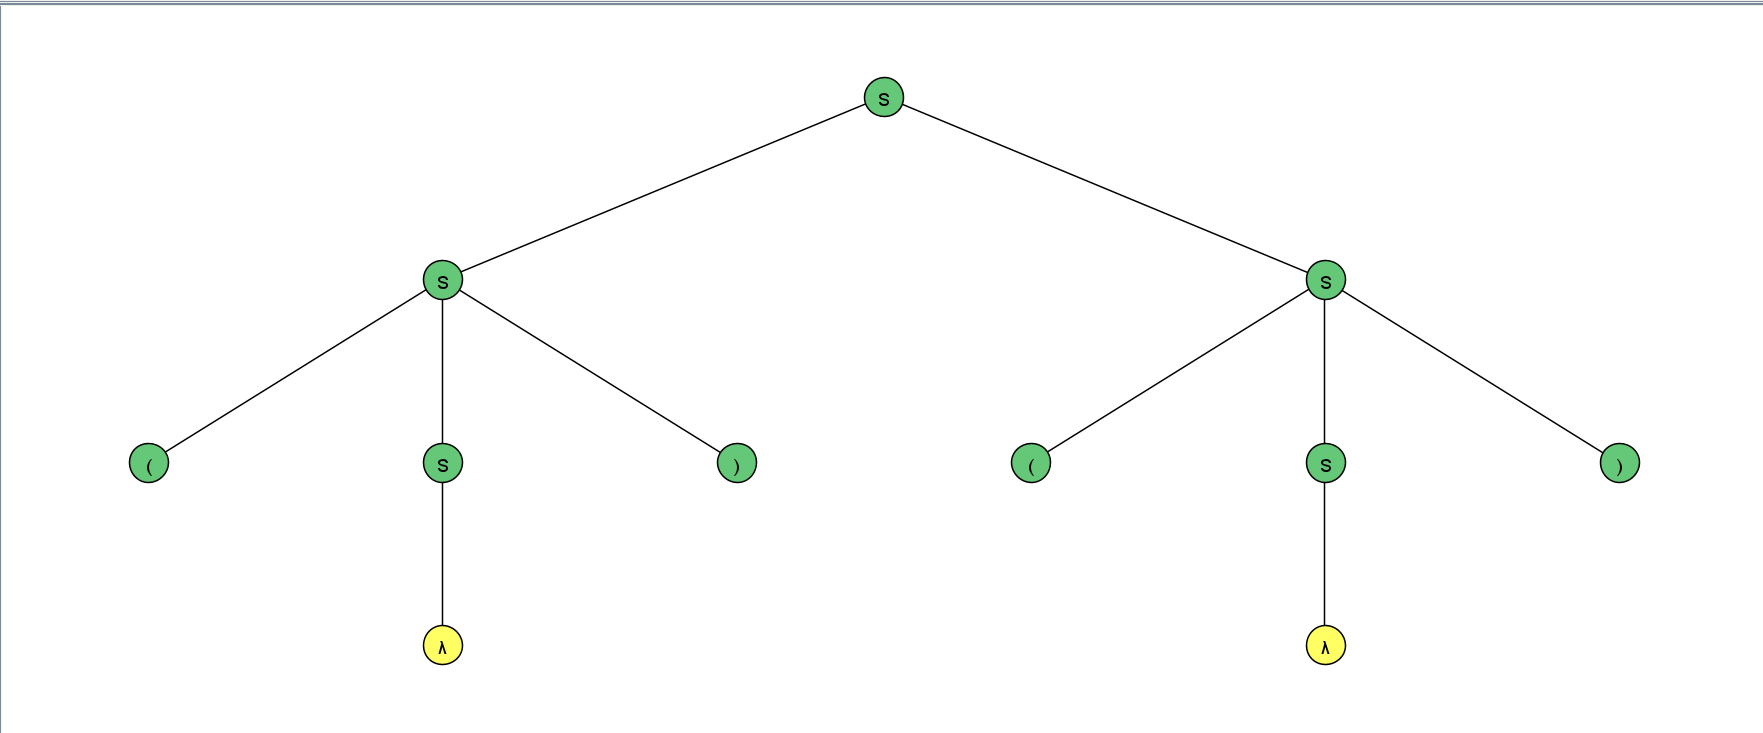
\includegraphics[width=1.0\textwidth]{syntaxtree_task7_1.png}\\
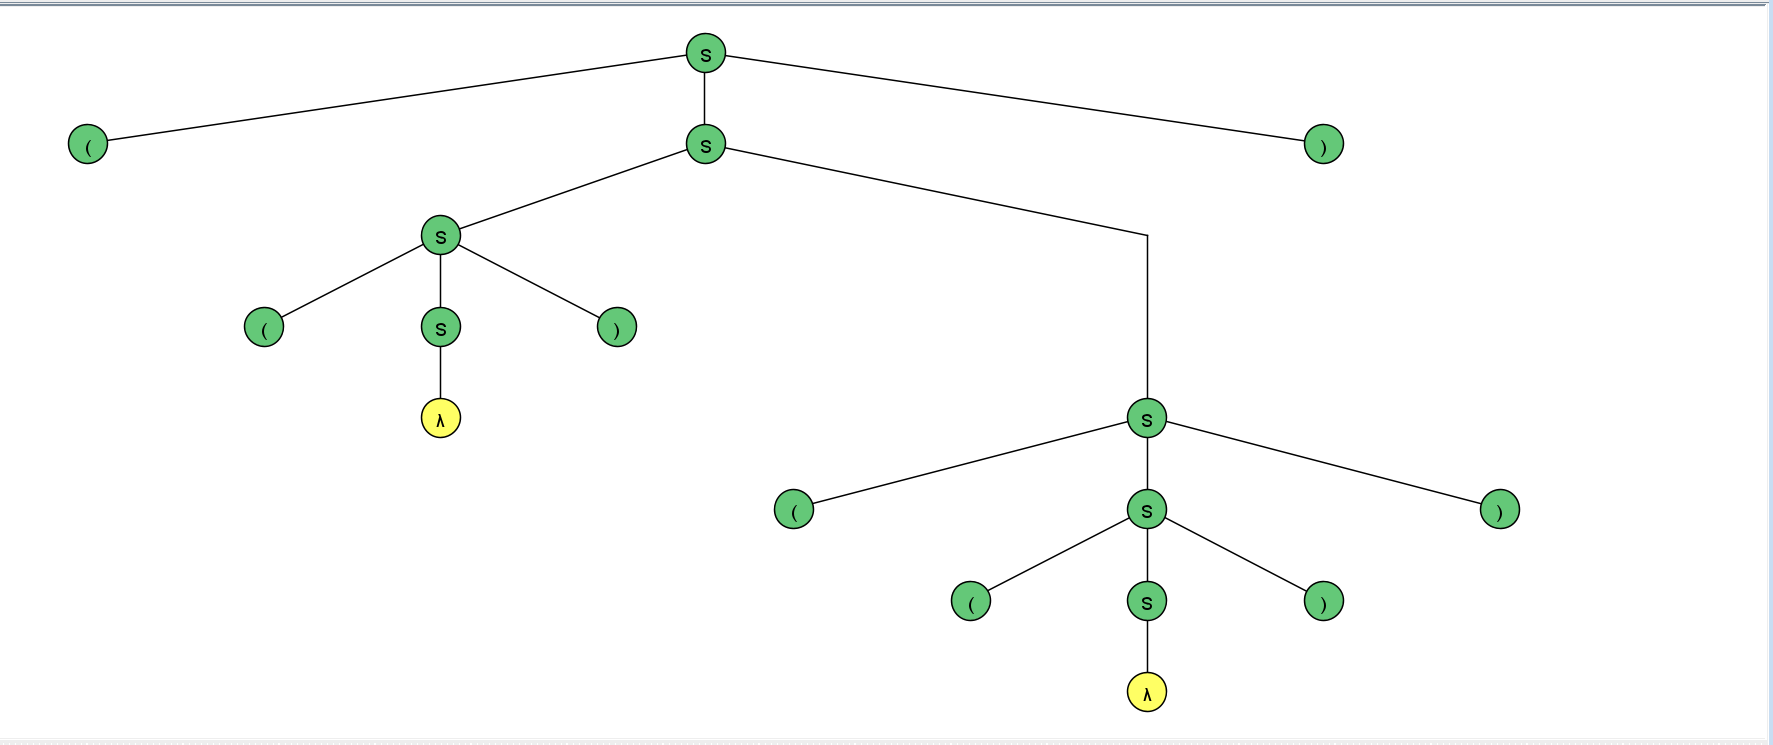
\includegraphics[width=1.0\textwidth]{syntaxtree_task7_2.png}\\
\section{Aufgabe}
\subsection{Grammatik}
Grammatik $G = (\{S, A, B\}, \{a-z, 0-9\}, P, S)\\
P = \{\\
S \rightarrow S+S\, |\, S*S\, |\, (S)\, |\, 1A\, |\, 2A\, |\, 3A\, |\, 4A\, |\, 5A\, |\, 6A\, |\, 7A\, |\, 8A\, |\, 9A\, |\, 0\, |\, B \\
A \rightarrow \epsilon\, |\, 0A\, |\, 1A\, |\, 2A\, |\, 3A\, |\, 4A\, |\, 5A\, |\, 6A\, |\, 7A\, |\, 8A\, |\, 9A\\
B \rightarrow BB\, |\, a\, |\, b\, |\, c\, |\, d\, |\, e\, |\, f\, |\, g\, |\, h\, |\, i\, |\, j\, |\, k\, |\, l\, |\, m\, |\, n\, |\, o\, |\, p\, |\, q\, |\, r\, |\, s\, |\, t\, |\, u\, |\, v\, |\, w\, |\, x\, |\, y\, |\, z\\
\}$
\subsection{Ableitungsbäume}
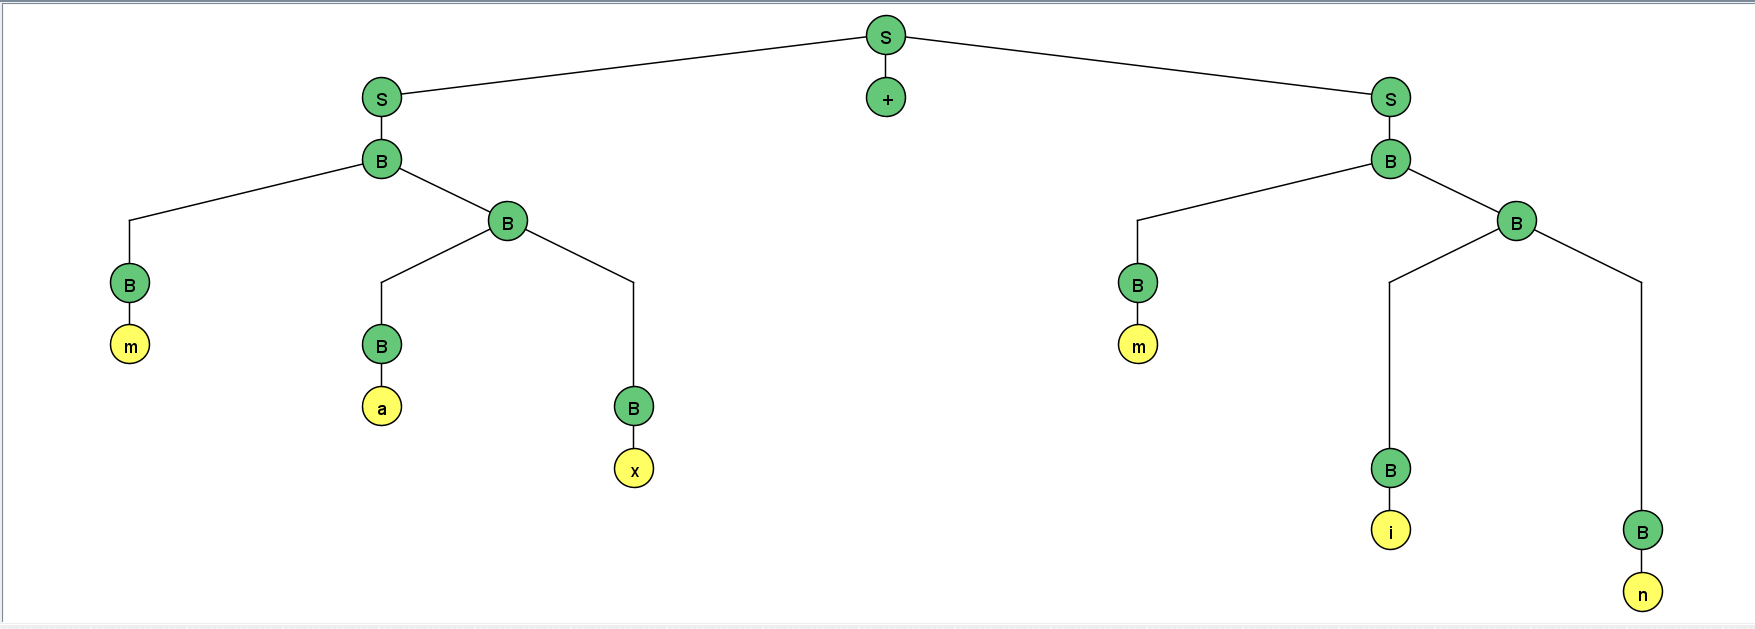
\includegraphics[width=1.0\textwidth]{syntaxtree_task8_1.png}\\
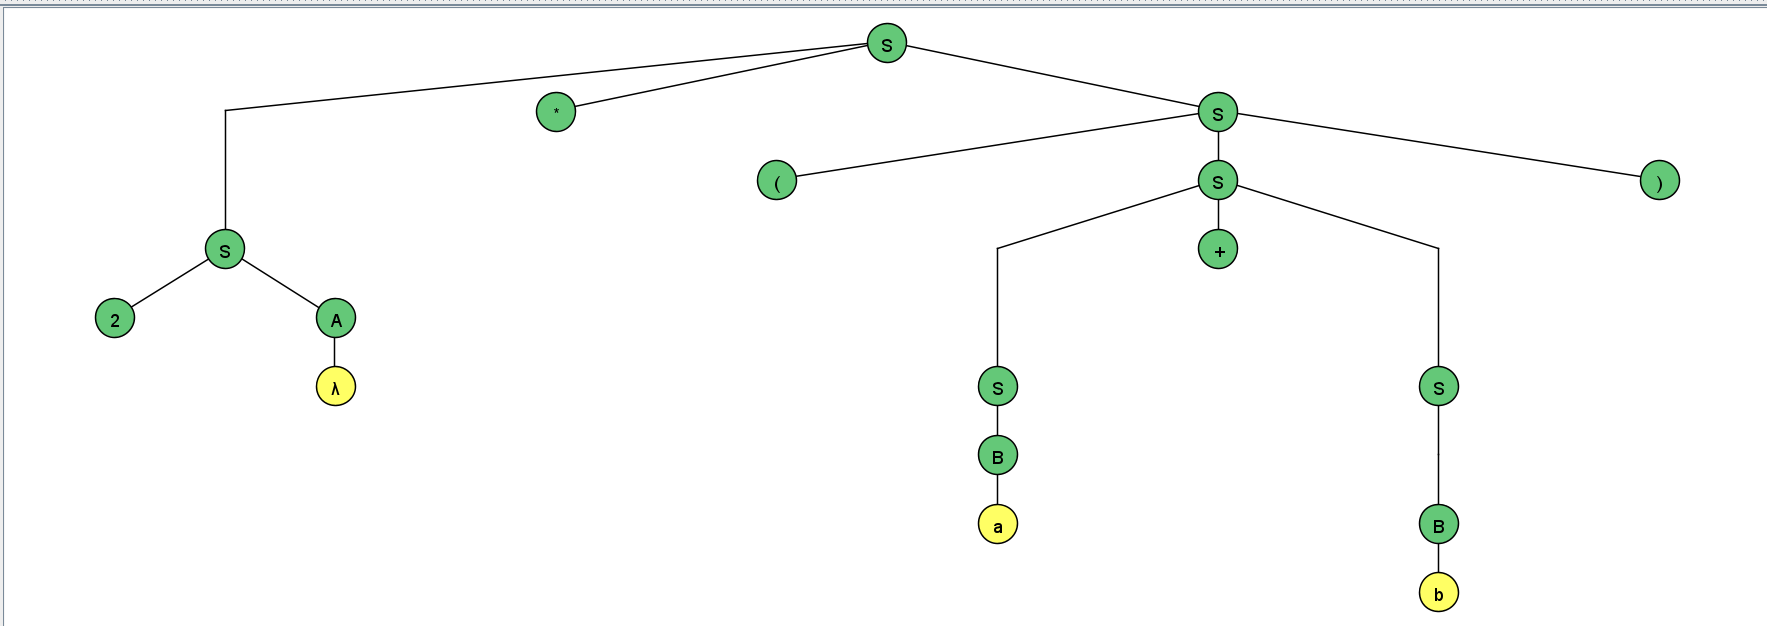
\includegraphics[width=1.0\textwidth]{syntaxtree_task8_2.png}\\
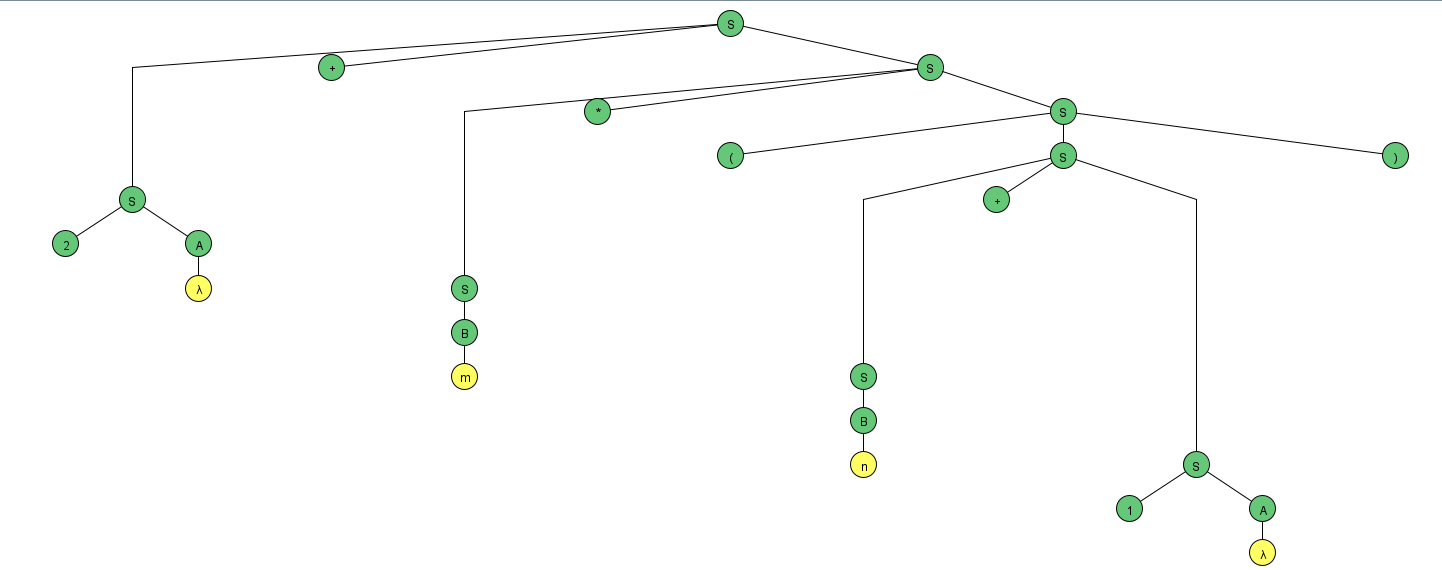
\includegraphics[width=1.0\textwidth]{syntaxtree_task8_3.png}\\
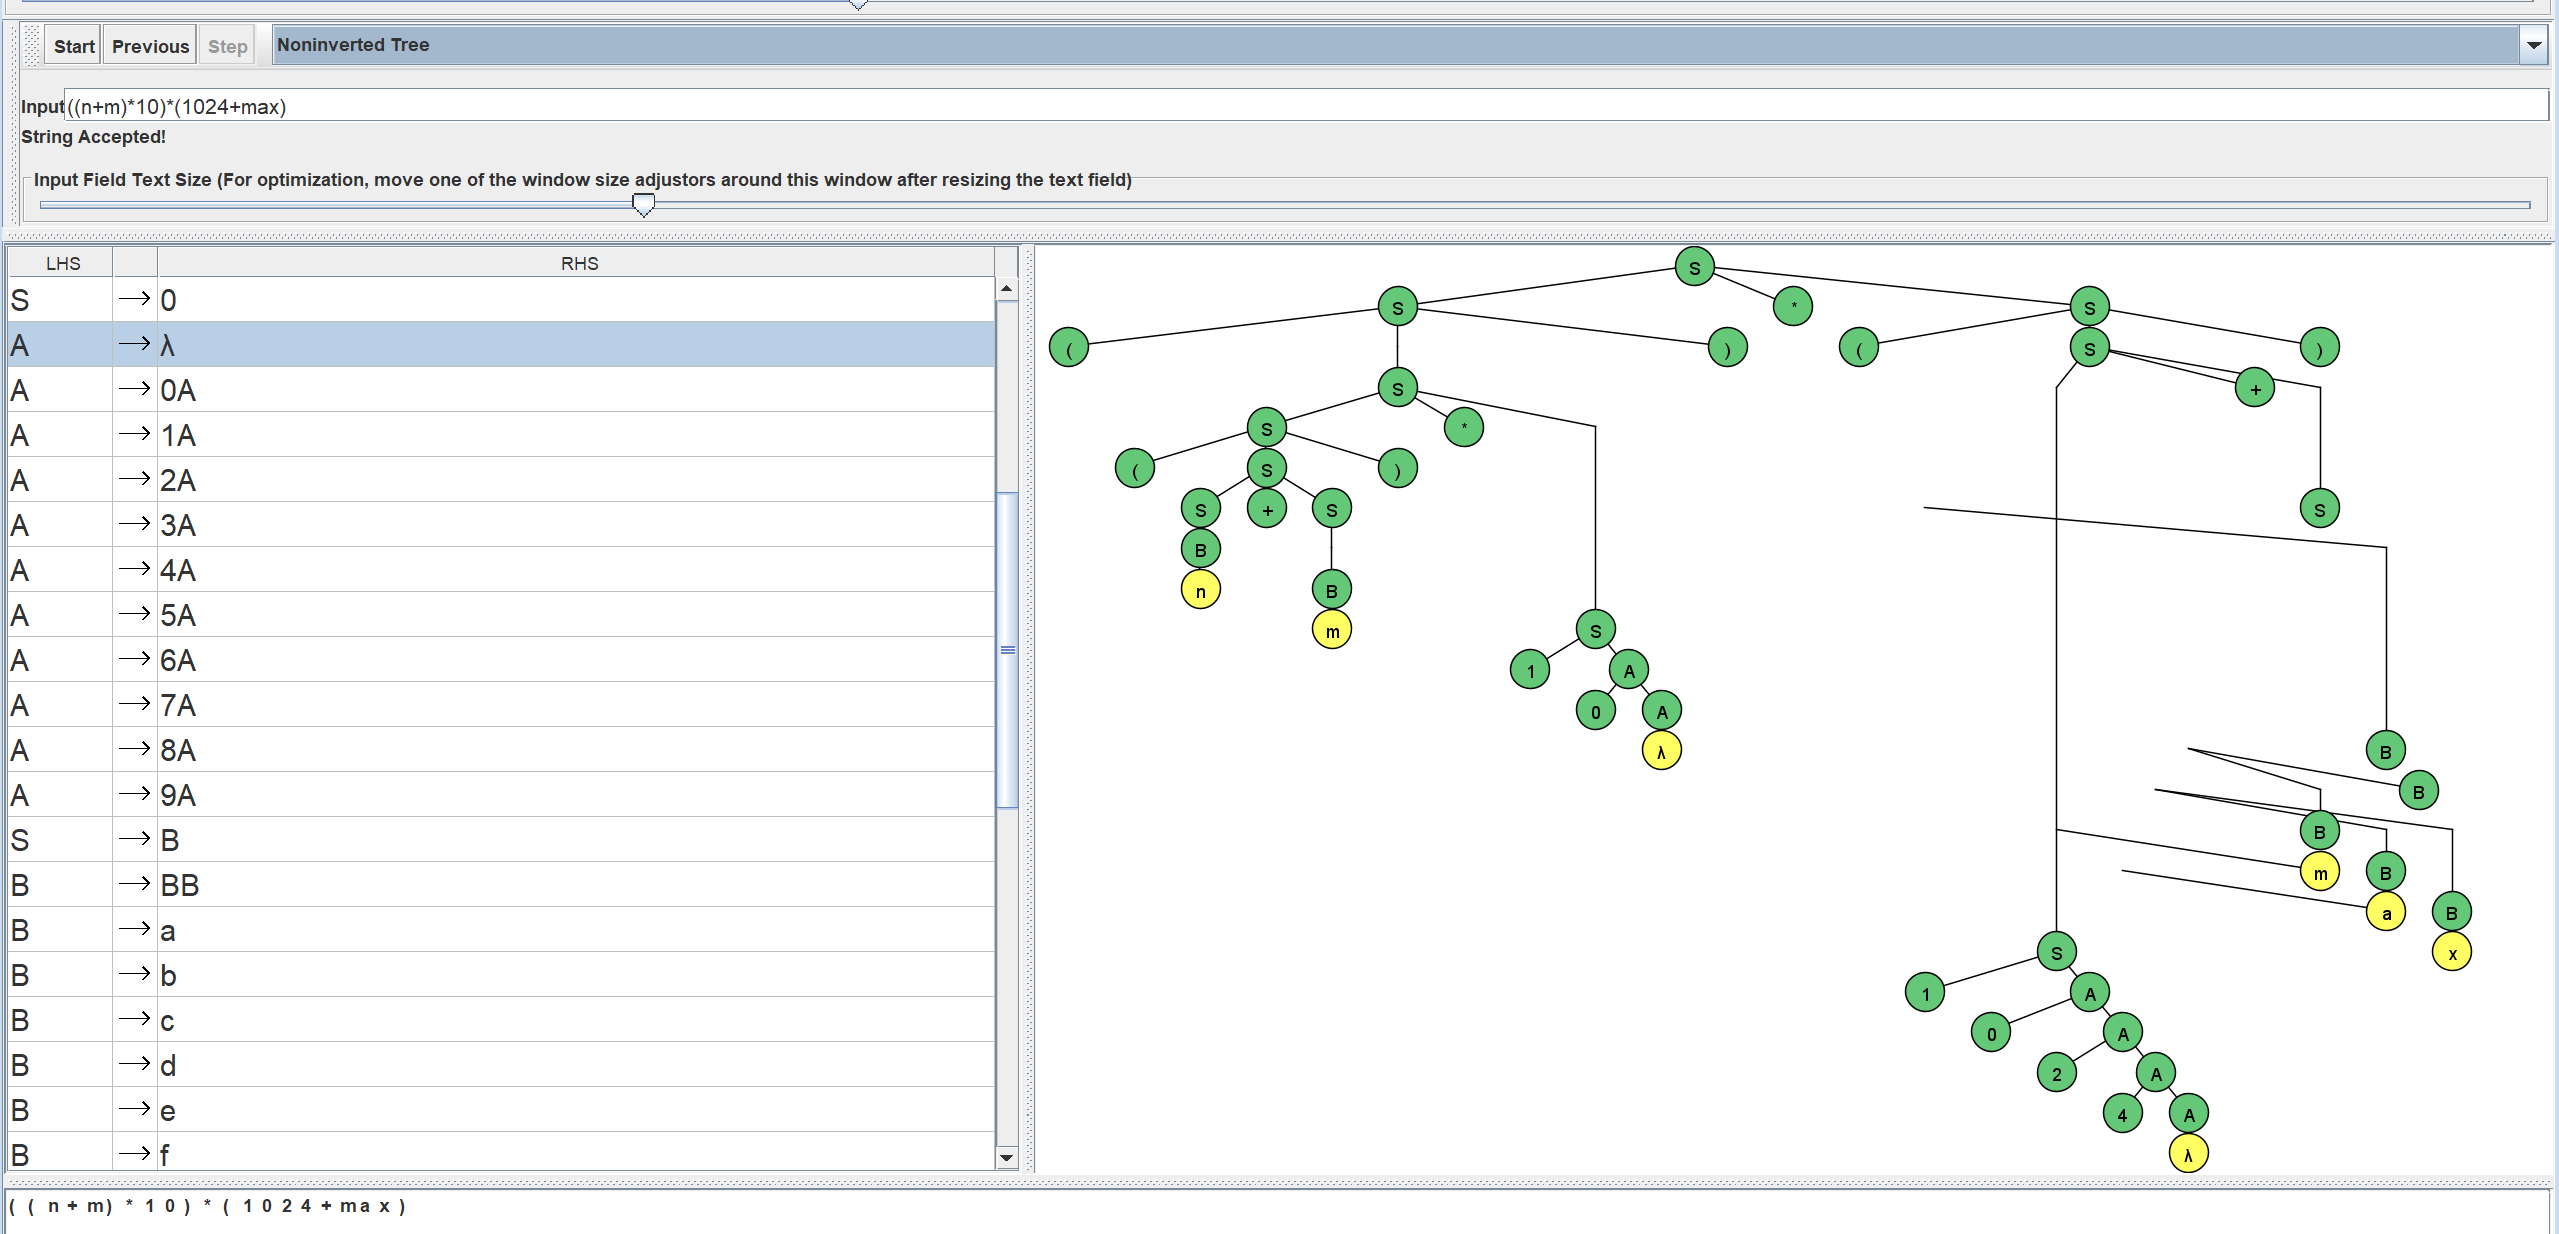
\includegraphics[width=1.0\textwidth]{syntaxtree_task8_4.png}\\
\section{Aufgabe}
\subsection{Herleiten von mindestens 5 Wörtern}
\begin{enumerate}
\item $S \Rightarrow bA \Rightarrow ba$
\item $S \Rightarrow aB \Rightarrow ab$
\item $S \Rightarrow bA \Rightarrow baS \Rightarrow babA \Rightarrow baba$
\item $S \Rightarrow aB \Rightarrow aaBB \Rightarrow aabB \Rightarrow aabb$
\item $S \Rightarrow bA \Rightarrow bbAA \Rightarrow bbaA \Rightarrow bbaa$
\end{enumerate}
\subsection{Syntaxbäume}
\subsubsection{Syntaxbaum von \glqq baabbbaa\grqq\, und von \glqq ababaabb\grqq}
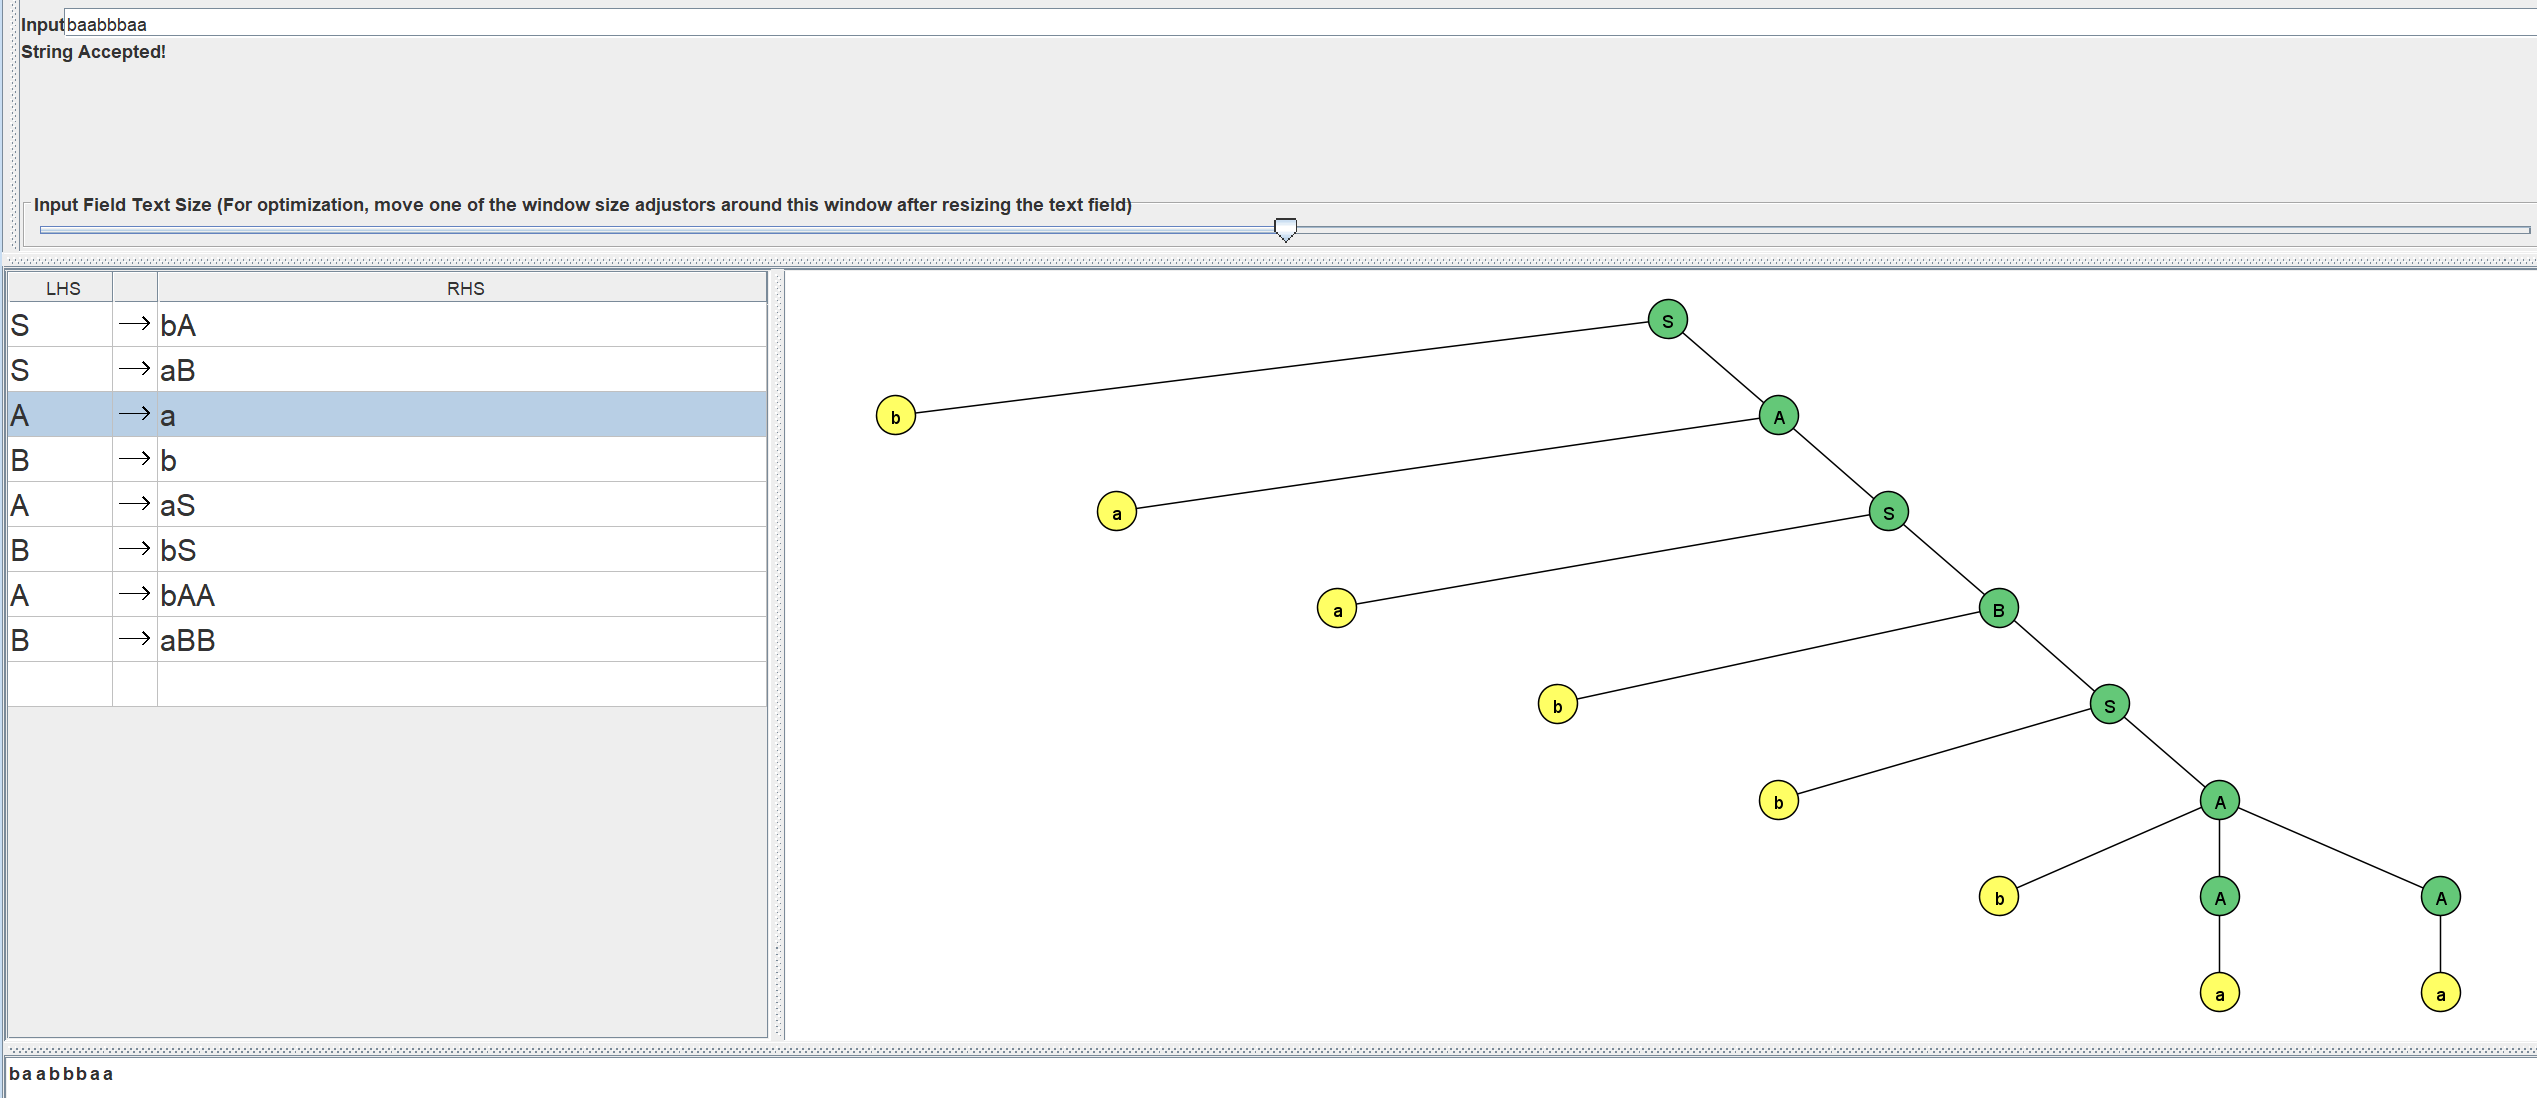
\includegraphics[width=1.0\textwidth]{syntaxtree_task9_1.png}\\
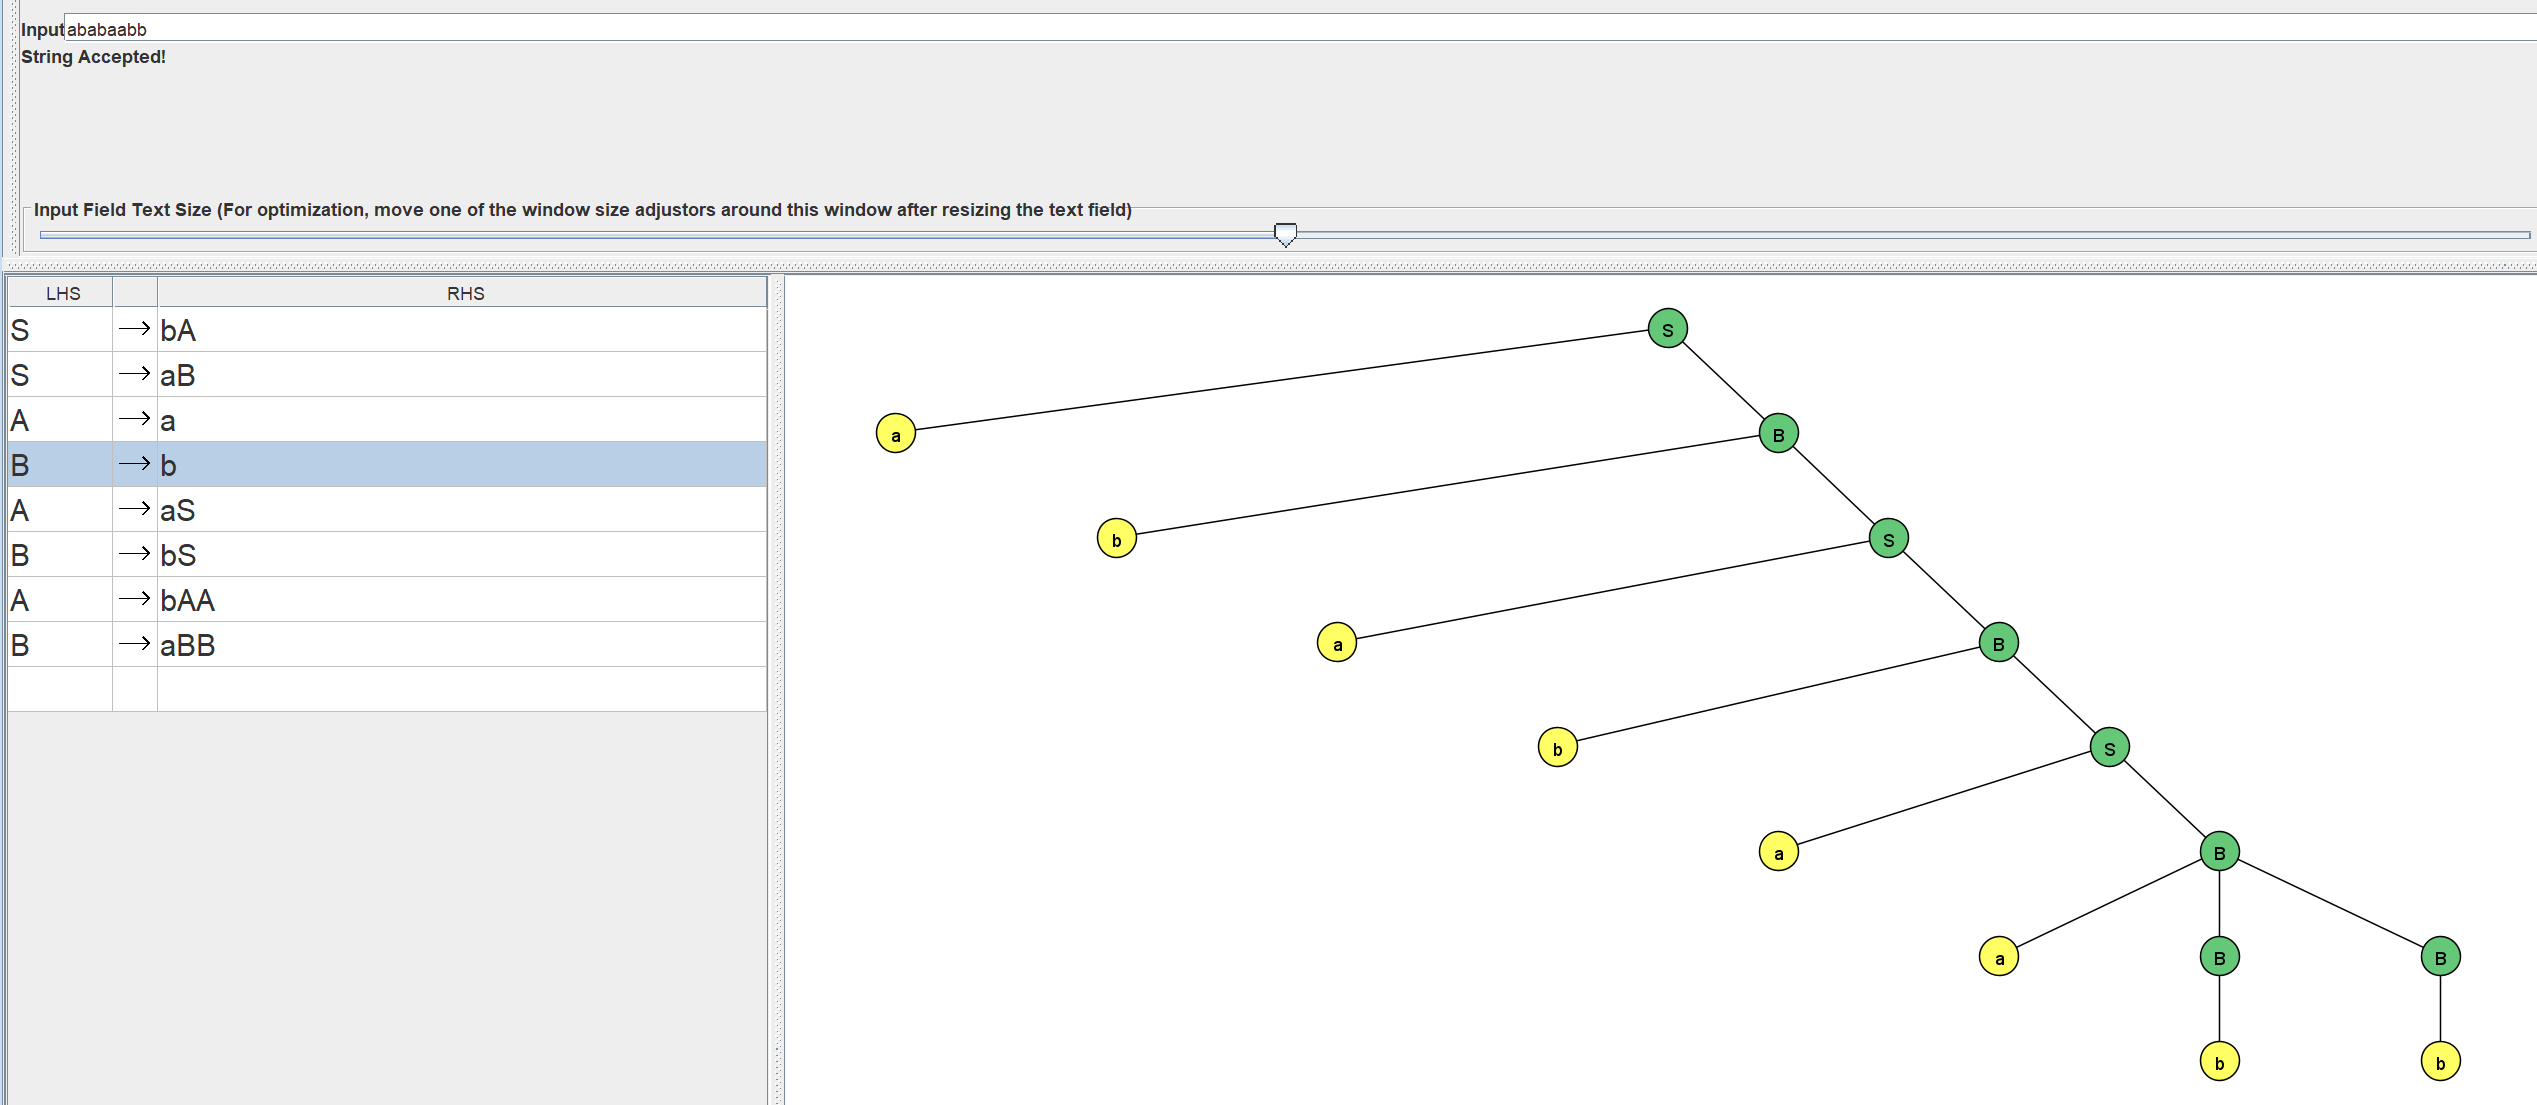
\includegraphics[width=1.0\textwidth]{syntaxtree_task9_2.png}\\
\subsubsection{Syntaxbäume von \glqq aababb\grqq}
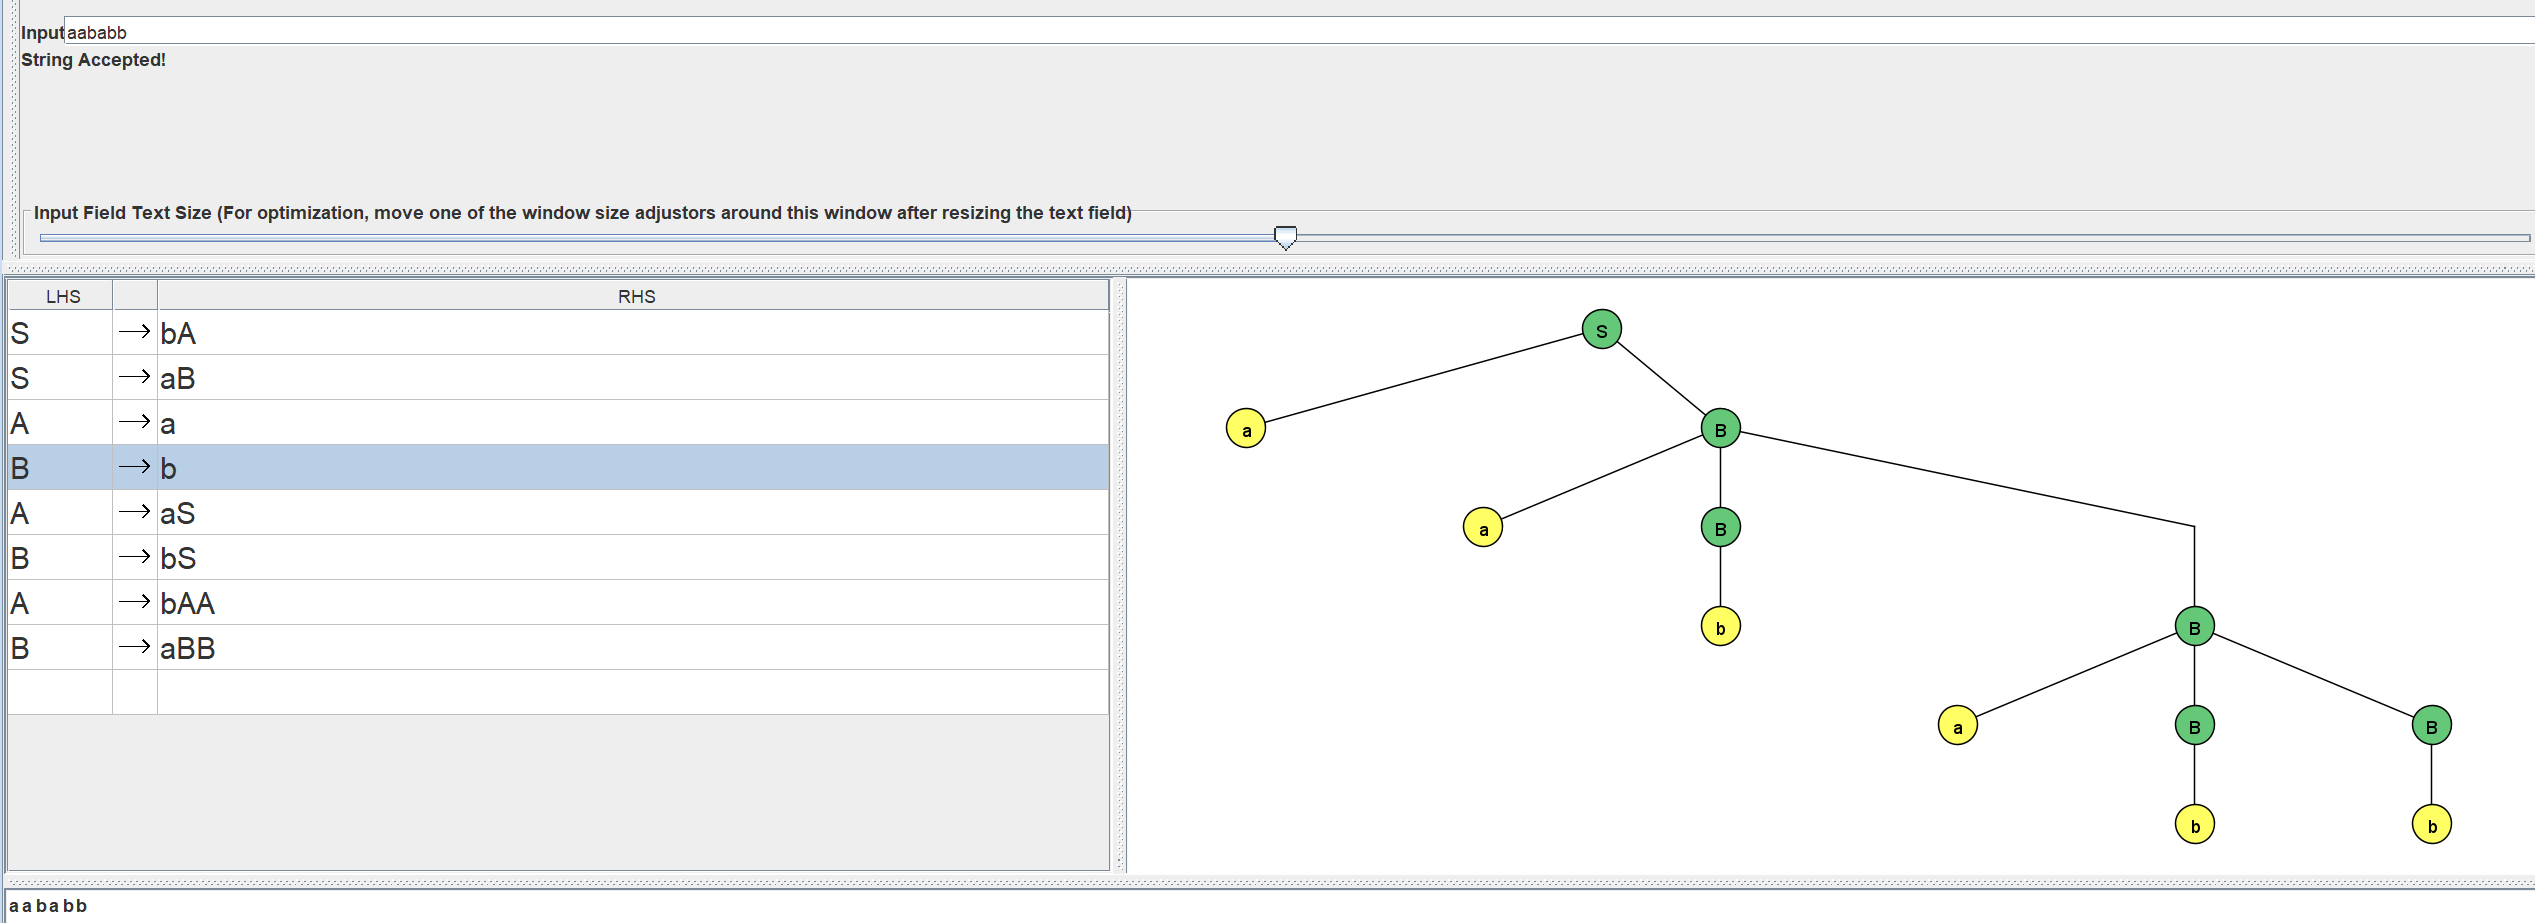
\includegraphics[width=1.0\textwidth]{syntaxtree_task9_3.png}\\
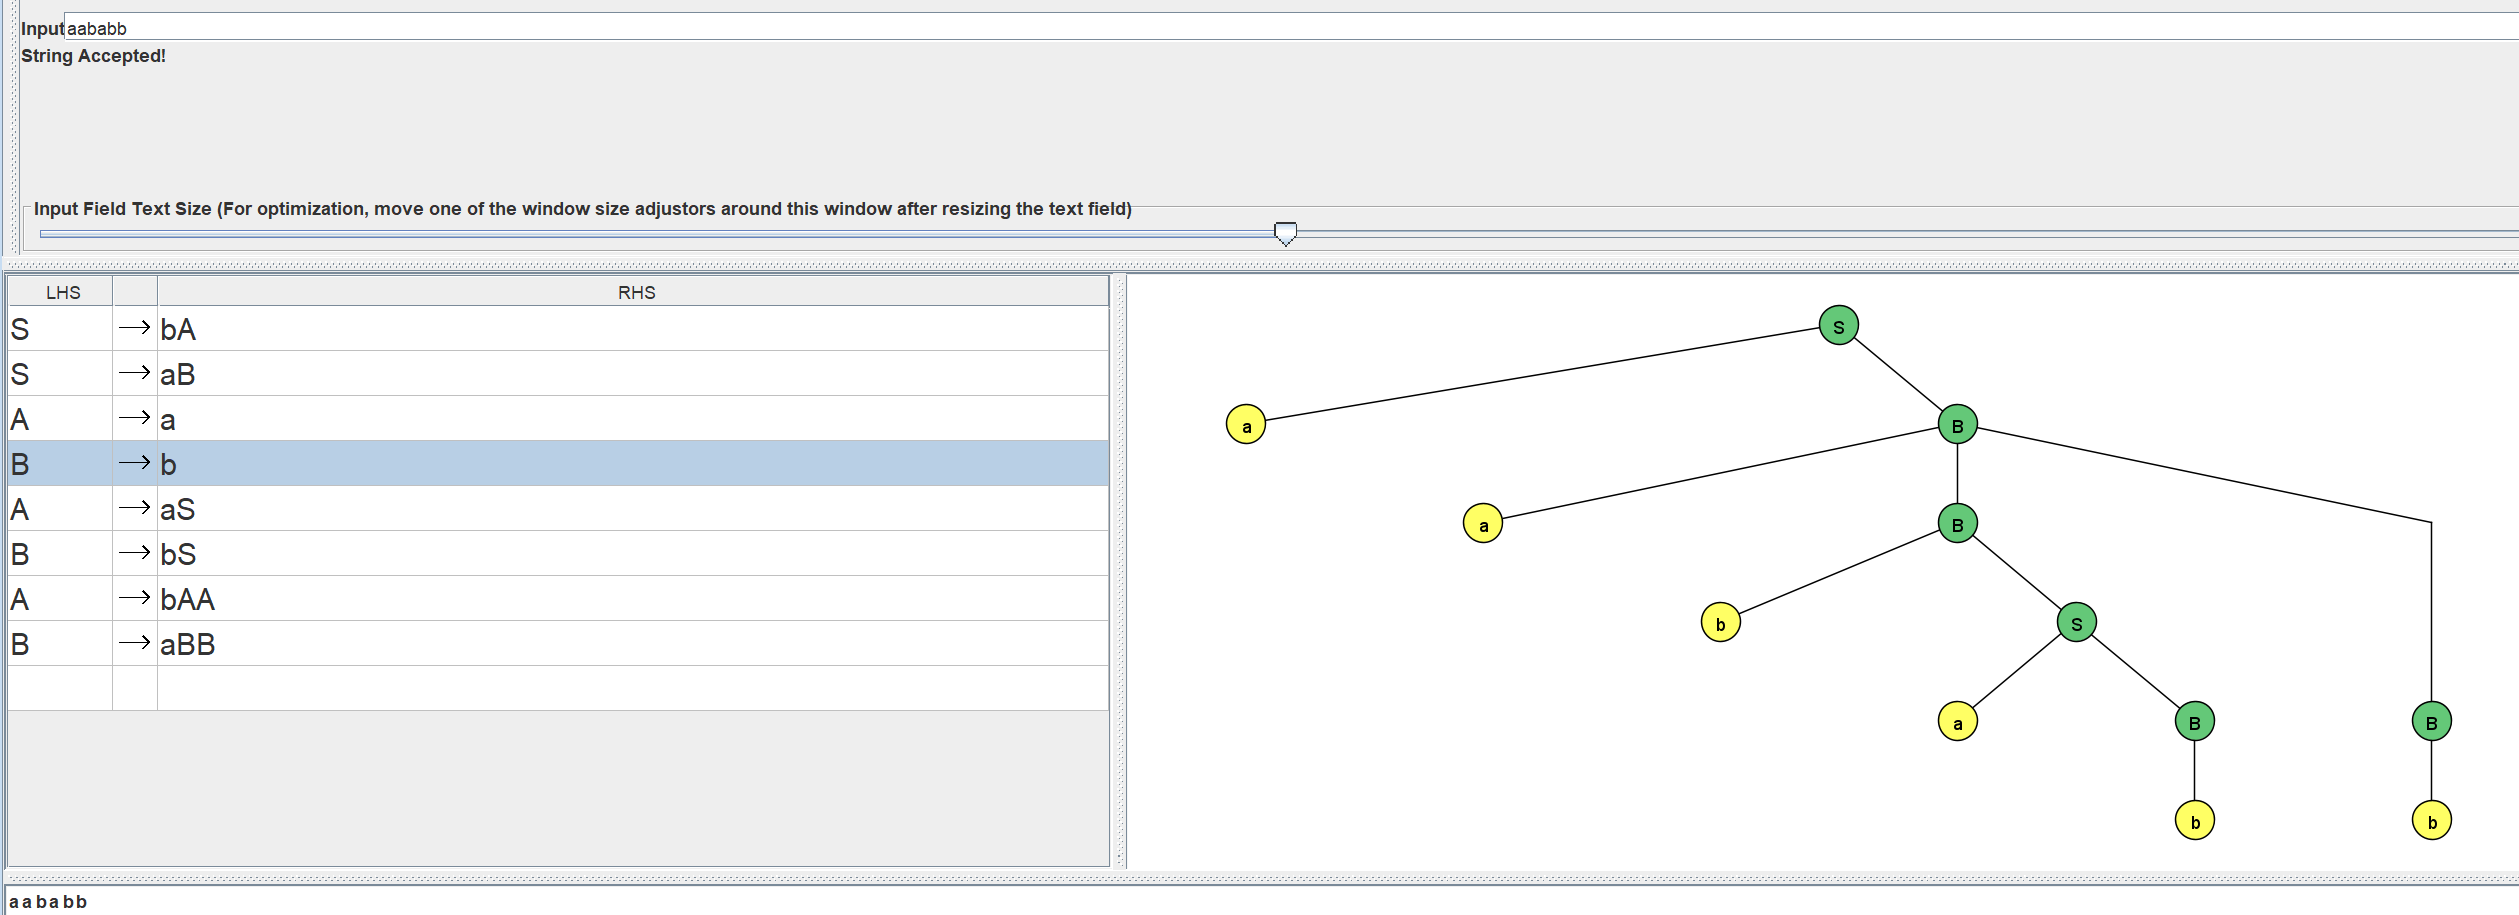
\includegraphics[width=1.0\textwidth]{syntaxtree_task9_4.png}\\
\subsection{Verbale Beschreibung von L(G)}
Jedes Wort der Sprache kann mit a oder b beginnen.\\
Jedes Wort der Sprache hat mindestens ein a und mindestens ein b.\\
Jedes Wort der Sprache hat gleich viele a wie b.\\
\end{document}
